\documentclass{article}
\usepackage{graphicx}
\usepackage{fontspec}
\setmainfont{Microsoft YaHei}
\usepackage{geometry}
\usepackage{ctex}
\usepackage{algorithm}  
\usepackage{algorithmicx}  
\usepackage{algpseudocode}  
\usepackage{amsmath}  
\title{HW10}
\author{王嵘晟 \quad PB1711614}
\date{}
\begin{document}
	\maketitle
	\section*{1.}
	\par{证书是从G1映射到G2,G1与它的图像同构。将G1和G2同构问题规约到团问题,为了检测图中是否有大小为k的团,让G1为K个顶点的完全图基础上的图,G2为原始图。如果能在多项式时间内解决子图同构问题,则可以在多项式时间内解决团问题。}
	\section*{2.}
	\par{为了证明哈密顿路径问题是NP完全的,首先证书为图中按顺序排列好的顶点的表$\{v_{1},v_{2},...,v_{n\}}$。可以在多项式时间内检查$(v_{i},v_{i+1}),1\le i\le n-1$是否是一条边。所以哈密顿路径问题是属于NP的。然后通过证明哈密顿回路问题$HAM-CYCLE\le_{P}HAM-PATH$。令G=(V,E)为任意图,按照以下方式建立G':对于每个$ e_{i}\in E$,令$G_{e_{i}}$表示顶集V,边集$E-e_{i}$的图。令$e_{i}$表示边$(u_{i},v_{i})$。这样对于每个$ e_{i}\in E$,G'包含$G_{e_{i}}$。此外G'还包含与$u_{1}$相连的顶x,一条从$v_{i}$到$u_{i+1}$的边,$1\le i\le |E|-1$,以及一个顶y,一套从$v_{|E|}$到y的边。从G构造G'可以在多项式时间内完成。如果图G有哈密顿圈,则对于每个i来说,$G_{e_{i}}$有从$u_{i}$开始到$v_{i}$结束的哈密顿路径。因此G'有从x开始到y结束的哈密顿圈,该圈通过依次经过这些哈密顿路径上的每一边得到。另一方面,假设G没有哈密顿循环。 由于x和y的度数为1,因此G'具有哈密顿路径的唯一可能是路径始于x并终止于y。此外,由于$(v_{1},u_{2})$为切边,如果存在必须在哈密顿圈里。由于不会第二次遍历这条边,任何哈密顿路径都必须以从x到$v_{1}$的哈密顿路径开始。但是,这意味着存在从$u_{1}$到$v_{1}$的哈密顿路径。由于($u_{1}$,$v_{1}$)是G中的一条边,这意味着G中存在哈密顿循环,这是一个矛盾。 因此,当且仅当G'具有哈密顿路径时,G具有哈密顿循环。因此HAM-PATH实际上是NP完整的。}
	\section*{3.}
	\par{由思考题23-3可知存在一种线性时间算法来计算图的瓶颈生成树,先运行此线性时间算法,以找到瓶颈树BT。然后遍历BT,最多连续跳过两个中间结点,遍历树中的每一个结点,这样可以获得一个有哈密顿圈的图,称为HB。用B来表示瓶颈生成树中最昂贵的边的成本,考虑每条不在BT中但在HB中的边的成本,由三角不等式,成本最多为3B。因为遍历单个边而不是通过最多3条边就可以从一个顶点到另一个。hb表示HB中成本最高的边,则$hb\le 3B$。所以HB中最贵的边顶多是3B,令B *表示最优瓶颈哈密顿游历HB *的最昂贵边的成本。 由于我们可以通过删除HB ∗中最昂贵的边来从HB ∗中获得生成树,因此任何生成树中最昂贵的边的最小成本小于或等于任何哈密顿圈中最昂贵的成本。所以$B\le B'$。由$hb\le 3B$,则$hb\le 3B'$。所以算法是3近似的。}
	\section*{4.}
	\subsection*{a.}
	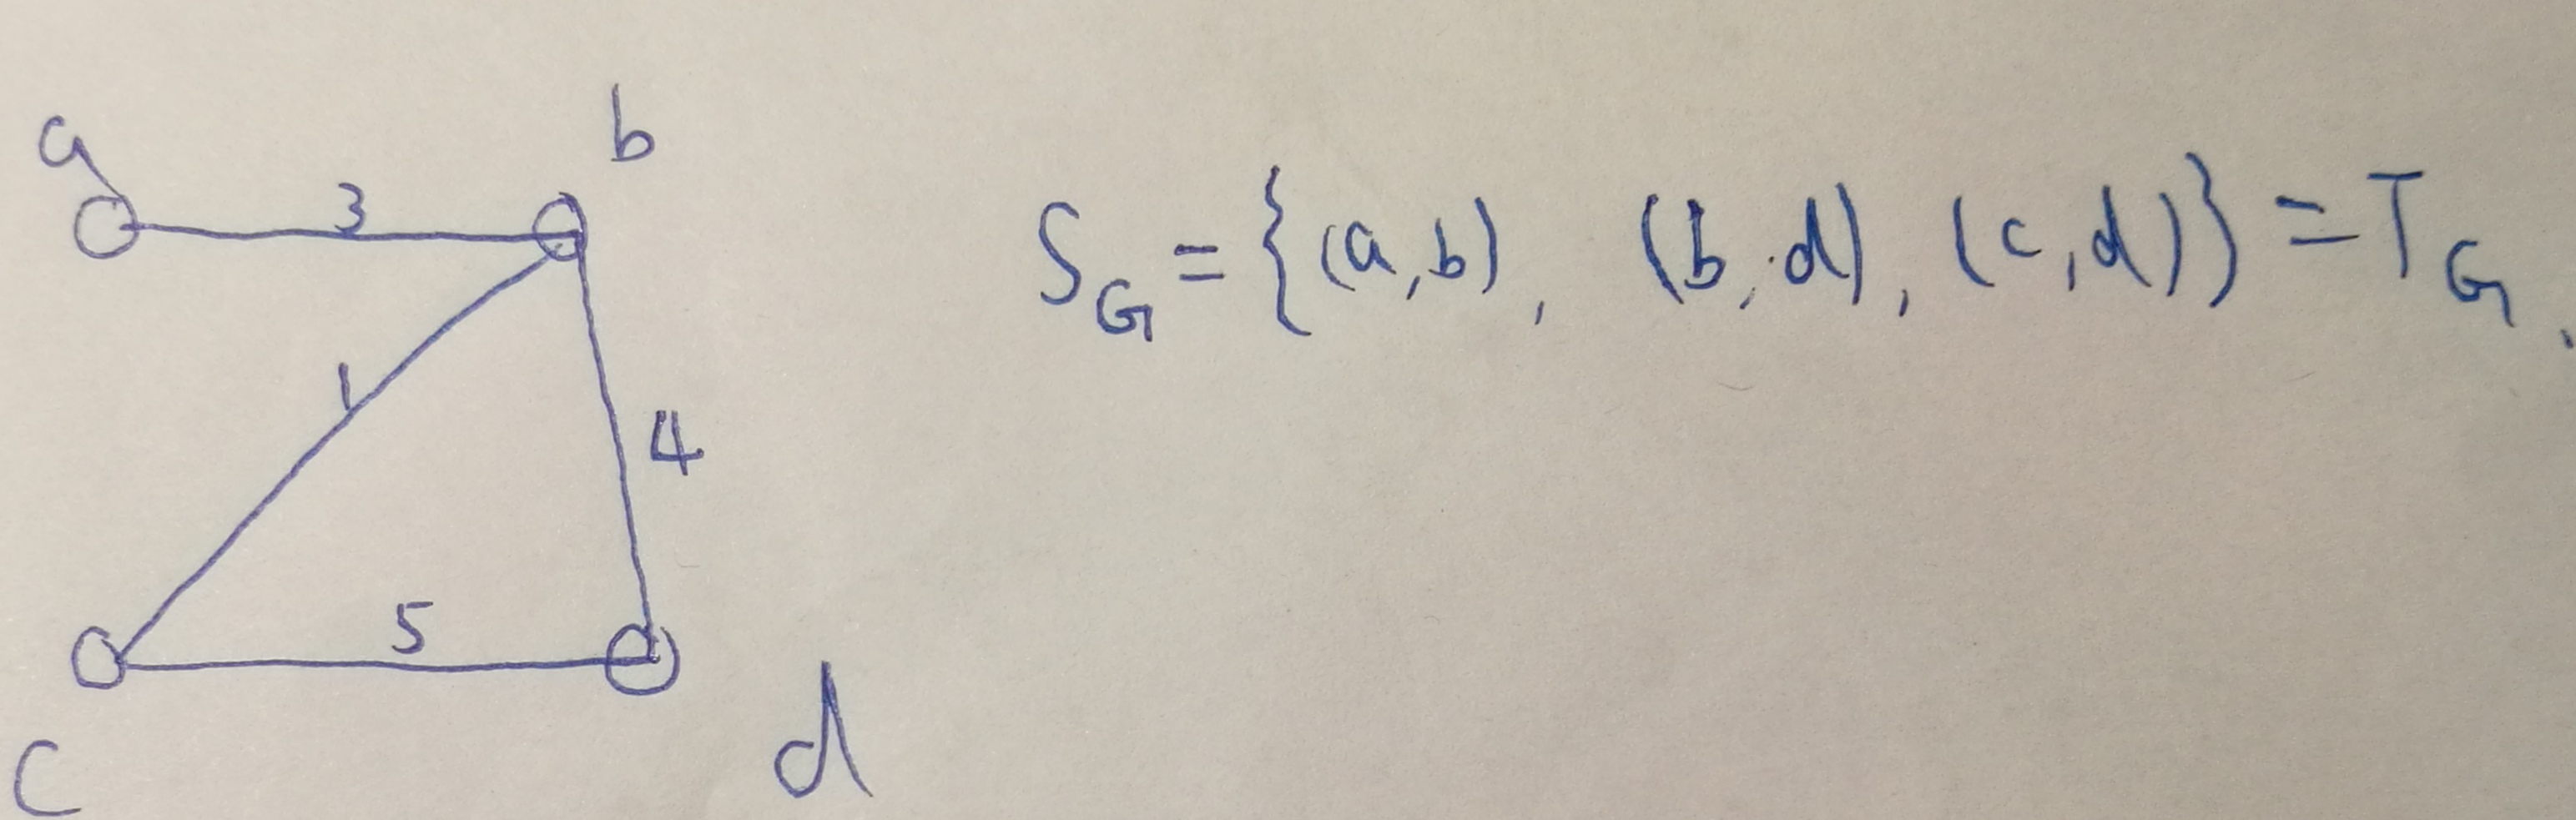
\includegraphics[scale=0.125]{1.jpg}
	\subsection*{b.}
	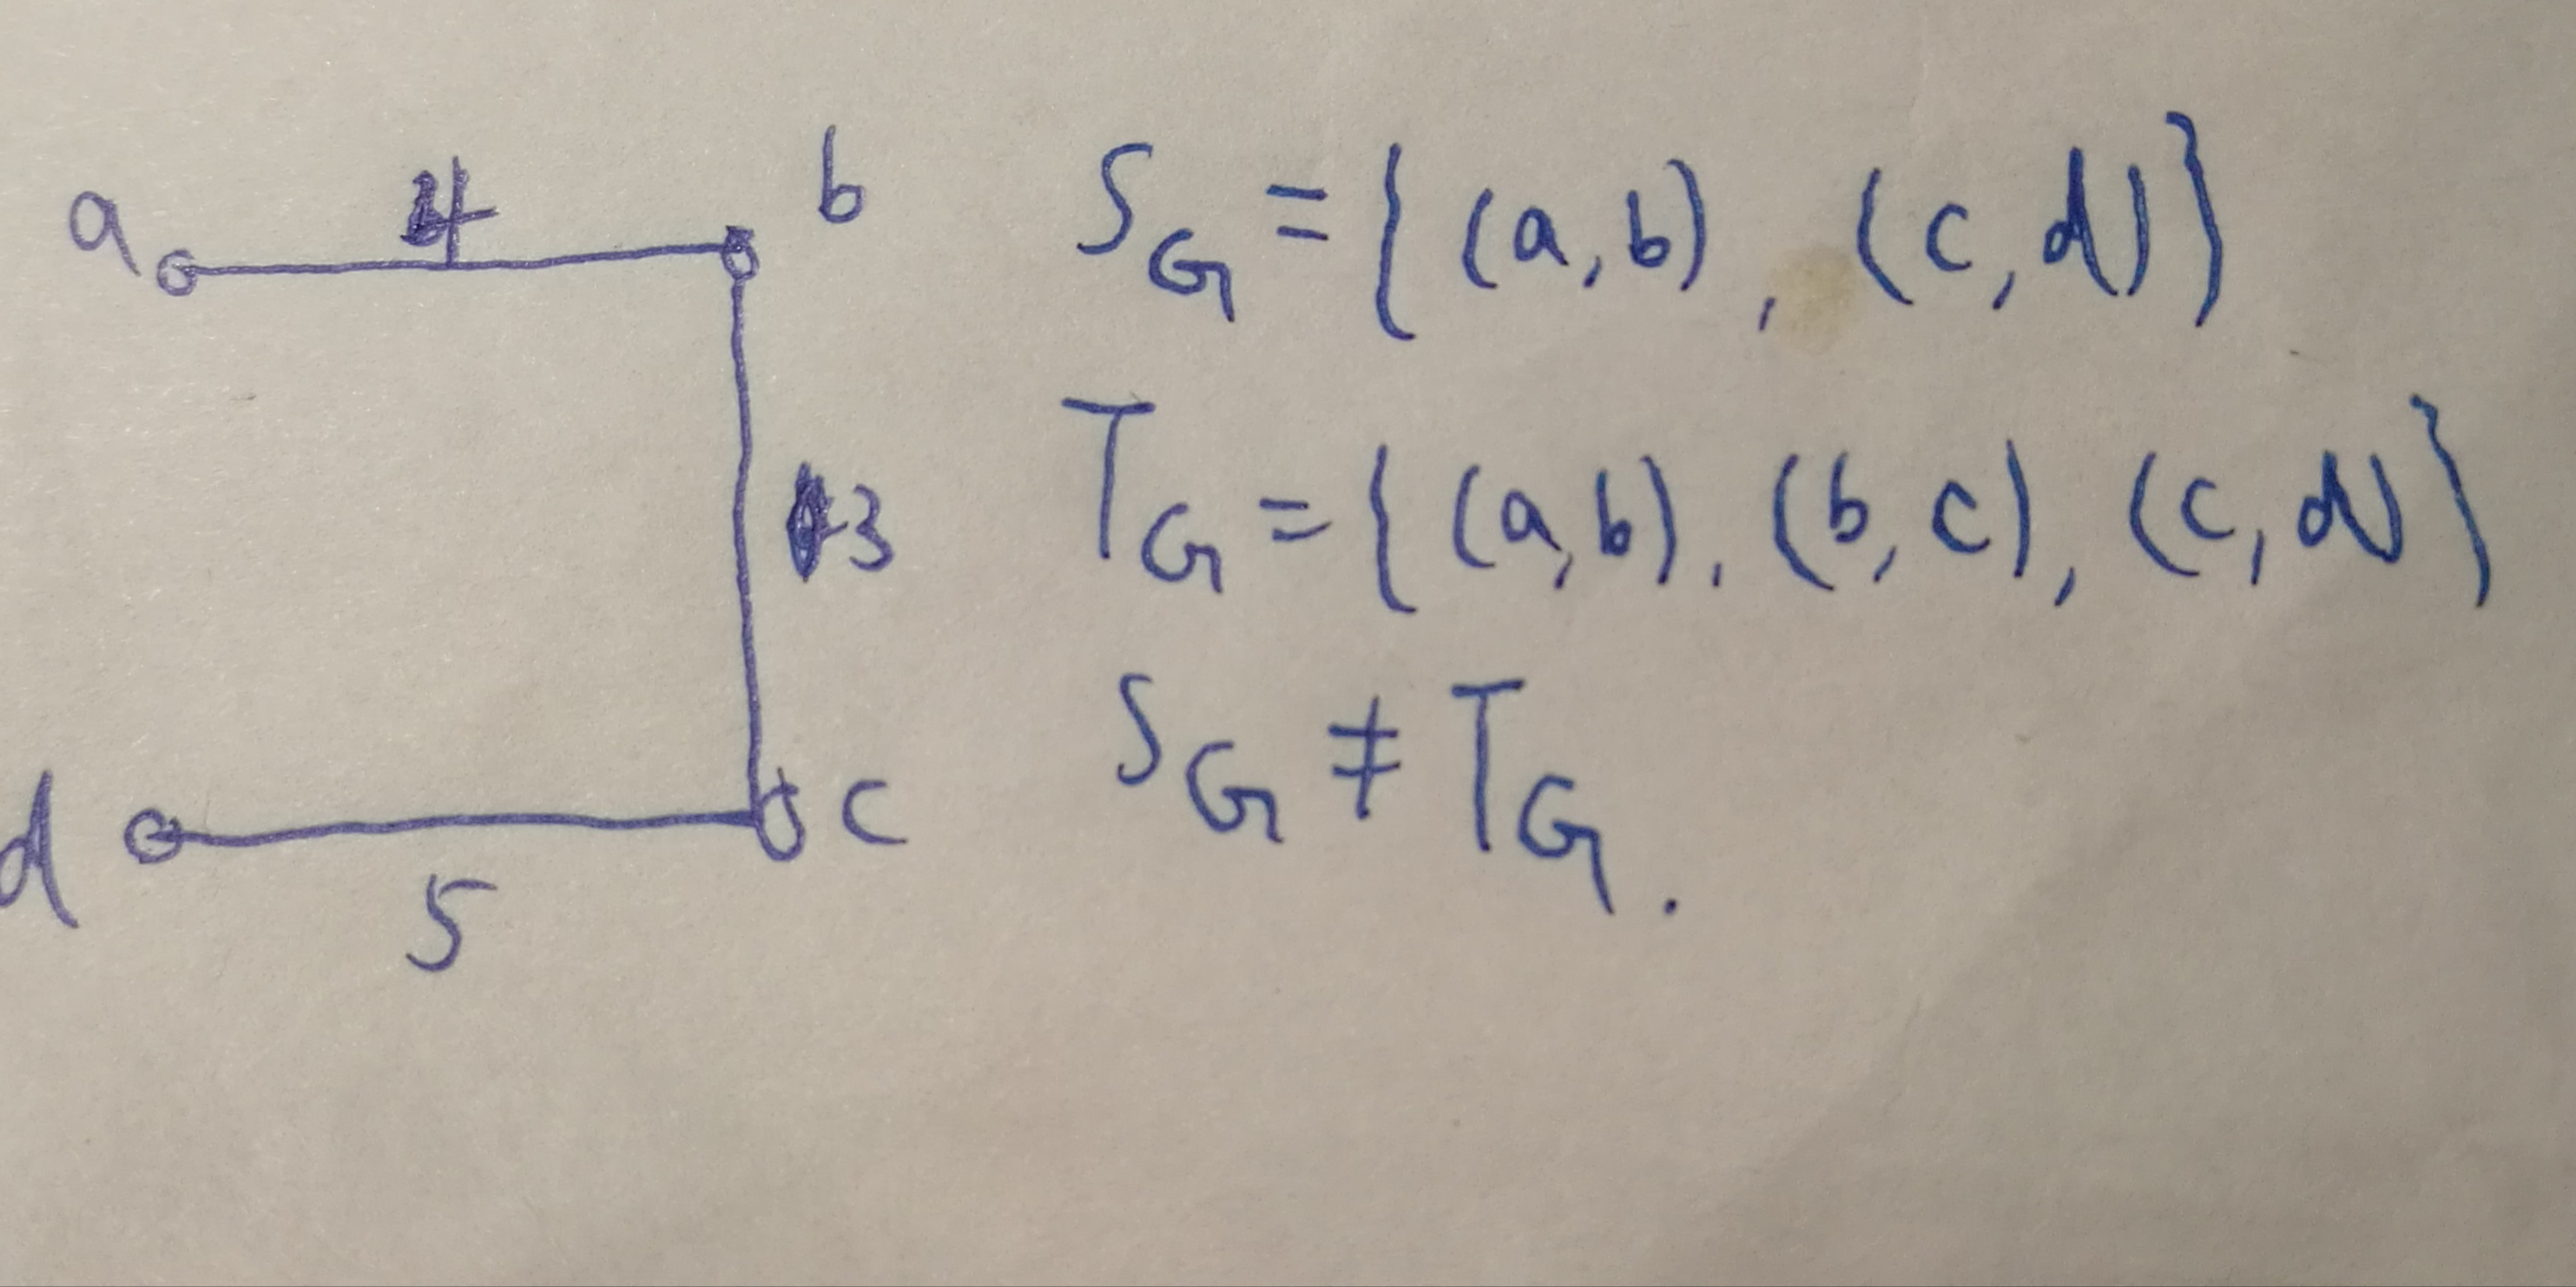
\includegraphics[scale=0.125]{2.jpg}
	\subsection*{c.}
	\par{用贪心算法来求最大权值生成树,将边由权值从大到小排序,如果边不会形成一个环路则将其加入树中。假设选择一条边(u,v)对u的权值最大,则边必然会引入一个环路,所以生成树中必然已经包含了边(w,u)。但由于向生成树中加边是按照权重递减的顺序的,所以$\omega(w,u)\textgreater \omega(u,v)$。这与(u,v)的权重最大矛盾。所以$S_{G}\subset T_{G}$。}
	\subsection*{d.}
	\par{由于每条边的权值都是不同的,因此特定的边可以是最多两个顶点的最大权值,所以$|S_{G}|\ge \frac{V}{2}$。所以$|T_{G}- S_{G}|\le |\frac{V}{2}|\le |S_{G}|$。由于$T_{G}-S_{G}$中每条边都不是最大权值的,每条边的权值都小于$S_{G}$中的任意一条边。令m为$S_{G}$中权值最小的边的权值,则$\omega(T_{G}-S_{G})\le m|S_{G}|$。所以$\omega(T_{G})\le \omega(S_{G})+m|S_{G}|\le 2\omega(S_{G})$所以$\omega(T_{G})\le \frac{\omega(S_{G})}{2}$}
	\subsection*{e.}
	\par{令N(v)表示结点v的邻结点,算法如下:}
	\begin{algorithm}
		\caption*{计算2近似的最大生成树}
		\begin{algorithmic}[1]
			\Function {APPROX-MAX-SPANNING-TREE} {$V,E$}
			\State	$T=\emptyset$
			\For  {$v\in V $}
				\State $max = -\infty$
				\State $best = v$
				\For {$u\in N(v)$}
					\If $\omega(u,v)\ge max$
						\State $v=u$
						\State $max=\omega(u,v)$
					\EndIf
				\EndFor
				\State $T=T\cup{u,v}$
			\EndFor
			\State\Return $T$
			\EndFunction
		\end{algorithmic}
	\end{algorithm}
	\section*{5.}
	\par{2-SAT问题是由两个布尔值组成的关系的集合,解决2-SAT问题可以通过对称性来解决。为每个需要被判定的量建立true、false两个节点,方便起见称它们为互斥节点,将约束条件抽象为代表推导关系的有向边。再由求强连通分量的Tarjan算法来缩点。若有一对互斥节点在同一强连通分量中则无解,将缩点后的森林中每条边反向,按照dfs序进行如下操作:初始时所有节点为无色,若当前节点未被染色,染成红色,然后将所有互斥点所在有向子树中的点全部染成黑色。否则什么都不做,继续处理下一个节点,可以证明上述操作不会使同一个节点被染上两种颜色。最终所有红色节点构成解集。时间复杂度O(V+E)}
\end{document}